\documentclass[runningheads,a4paper]{llncs}

%\usepackage[spanish]{babel}
\usepackage{amssymb}
\setcounter{tocdepth}{3}
\usepackage{graphicx}

\usepackage{color}
\usepackage{listings}
\definecolor{mygreen}{rgb}{0,0.6,0}
\lstdefinestyle{python}{language=[Python],  rulecolor=\color{blue!80!black}}
\lstset{language = csh, language = python, basicstyle = \bfseries\ttfamily, keywordstyle = \color{blue}, commentstyle=\color{mygreen}, breaklines = true, showstringspaces=false}
\usepackage{xcolor, pstricks}
\usepackage{multicol}

\usepackage[spanish]{babel}
\usepackage[pdftex]{hyperref}

\usepackage{url}
\urldef{\mailsa}\path|{amalia.ibarra, gabriela.martinez}@estudiantes.matcom.uh.cu|      
\newcommand{\keywords}[1]{\par\addvspace\baselineskip
\noindent\keywordname\enspace\ignorespaces#1}


\begin{document}
\renewcommand{\abstractname}{Resumen.}
\renewcommand{\keywordname}{\textbf{Palabras Clave:}}
\renewcommand{\refname}{Referencias}
\renewcommand{\tablename}{Tabla}

\mainmatter  % start of an individual contribution

\title{Proyecto de Prolog.\\Juego Hive.}

\titlerunning{Prolog-Hive}

\author{Amalia Ibarra Rodr\'iguez\\
	Gabriela B. Mart\'inez Giraldo}

\authorrunning{Amalia et al.}

\institute{Universidad de La Habana,\\La Habana, Cuba\\
Grupo C-412\\
\mailsa\\}
\maketitle


\section{Descripción del problema}\label{sec:ex1}

\begin{figure}
	\centering
	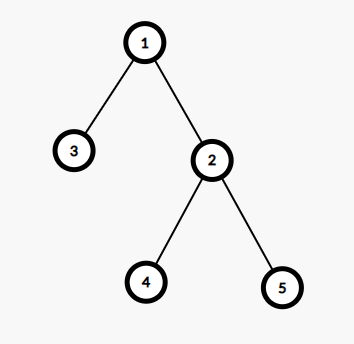
\includegraphics[width = 8cm]{images/lcc1.png}
	\caption{Grafo cuyo centroide es el v\'ertice 2.}\label{fig:lcc1}
\end{figure}


\subsection{Idea seguida}


\begin{center}
	\begin{lstlisting}
	def dfs_centroids(vertex, parent):
	   size[vertex] = 1
	   is_centroid = True
	   edge = (parent, vertex)
	
	   for adj in graph[vertex]:
	      if adj != parent:
	         last_edge = dfs(adj, vertex)
	         size[vertex] += size[adj]
	         edge = last_edge
	
	         if size[adj] > n / 2:
	            is_centroid = False
	
	   if n - size[vertex] > n / 2:
	      is_centroid = False
	   if is_centroid:
	      centroids.append([vertex, *last_edge])
	
	   return edge
	\end{lstlisting}
\end{center} 

\begin{thebibliography}{99}
	\bibitem{cf} CodeForces Problem 1406 C Link Cut Centroids: \href{https://codeforces.com/contest/1406/problem/C}
	{https://codeforces.com/contest/1406/problem/C}.
\end{thebibliography}

\end{document}
